%%%%%%%%%%%%%%%%%%%%%%%%%%%%%%%%%%%%%%%%%
% Wenneker Article
% LaTeX Template
% Version 2.0 (28/2/17)
%
% This template was downloaded from:
% http://www.LaTeXTemplates.com
%
% Authors:
% Vel (vel@LaTeXTemplates.com)
% Frits Wenneker
%
% License:
% CC BY-NC-SA 3.0 (http://creativecommons.org/licenses/by-nc-sa/3.0/)
%
% Adapted for COMS30007 by Carl Henrik Ek
%
%%%%%%%%%%%%%%%%%%%%%%%%%%%%%%%%%%%%%%%%%

%----------------------------------------------------------------------------------------
%	PACKAGES AND OTHER DOCUMENT CONFIGURATIONS
%----------------------------------------------------------------------------------------

\documentclass[10pt, a4paper, twocolumn]{article} % 10pt font size (11 and 12 also possible), A4 paper (letterpaper for US letter) and two column layout (remove for one column)

%%%%%%%%%%%%%%%%%%%%%%%%%%%%%%%%%%%%%%%%%
% Wenneker Article
% Structure Specification File
% Version 1.0 (28/2/17)
%
% This file originates from:
% http://www.LaTeXTemplates.com
%
% Authors:
% Frits Wenneker
% Vel (vel@LaTeXTemplates.com)
%
% License:
% CC BY-NC-SA 3.0 (http://creativecommons.org/licenses/by-nc-sa/3.0/)
%
% Adapted for COMS30007 by Carl Henrik Ek
%
%%%%%%%%%%%%%%%%%%%%%%%%%%%%%%%%%%%%%%%%%

%----------------------------------------------------------------------------------------
%	PACKAGES AND OTHER DOCUMENT CONFIGURATIONS
%----------------------------------------------------------------------------------------

\usepackage[english]{babel} % English language hyphenation

\usepackage{microtype} % Better typography

\usepackage{amsthm} % Math packages for equations
\usepackage{amsmath}
\usepackage{amssymb}
\usepackage{mathtools}
\usepackage{bm}
\usepackage{xfrac}
\usepackage{resizegather}
\usepackage[backend=bibtex,style=numeric]{biblatex}



\usepackage[svgnames]{xcolor} % Enabling colors by their 'svgnames'

\usepackage[hang, small, labelfont=bf, up, textfont=it]{caption} % Custom captions under/above tables and figures

\usepackage{booktabs} % Horizontal rules in tables

\usepackage{lastpage} % Used to determine the number of pages in the document (for "Page X of Total")

\usepackage{graphicx} % Required for adding images

\usepackage{enumitem} % Required for customising lists
\setlist{noitemsep} % Remove spacing between bullet/numbered list elements

\usepackage{sectsty} % Enables custom section titles
\allsectionsfont{\usefont{OT1}{phv}{b}{n}} % Change the font of all section commands (Helvetica)

%----------------------------------------------------------------------------------------
%	MARGINS AND SPACING
%----------------------------------------------------------------------------------------

\usepackage{geometry} % Required for adjusting page dimensions

\geometry{
	top=1cm, % Top margin
	bottom=1.5cm, % Bottom margin
	left=2cm, % Left margin
	right=2cm, % Right margin
	includehead, % Include space for a header
	includefoot, % Include space for a footer
	%showframe, % Uncomment to show how the type block is set on the page
}

\setlength{\columnsep}{7mm} % Column separation width

%----------------------------------------------------------------------------------------
%	FONTS
%----------------------------------------------------------------------------------------

\usepackage[T1]{fontenc} % Output font encoding for international characters
\usepackage[utf8]{inputenc} % Required for inputting international characters

\usepackage{XCharter} % Use the XCharter font

%----------------------------------------------------------------------------------------
%	HEADERS AND FOOTERS
%----------------------------------------------------------------------------------------

\usepackage{fancyhdr} % Needed to define custom headers/footers
\pagestyle{fancy} % Enables the custom headers/footers

\renewcommand{\headrulewidth}{0.0pt} % No header rule
\renewcommand{\footrulewidth}{0.4pt} % Thin footer rule

\renewcommand{\sectionmark}[1]{\markboth{#1}{}} % Removes the section number from the header when \leftmark is used

%\nouppercase\leftmark % Add this to one of the lines below if you want a section title in the header/footer

% Headers
\lhead{} % Left header
\chead{\textit{\thetitle}} % Center header - currently printing the article title
\rhead{} % Right header

% Footers
\lfoot{} % Left footer
\cfoot{} % Center footer
\rfoot{\footnotesize Page \thepage\ of \pageref{LastPage}} % Right footer, "Page 1 of 2"

\fancypagestyle{firstpage}{ % Page style for the first page with the title
	\fancyhf{}
	\renewcommand{\footrulewidth}{0pt} % Suppress footer rule
}

%----------------------------------------------------------------------------------------
%	TITLE SECTION
%----------------------------------------------------------------------------------------

\newcommand{\authorstyle}[1]{{\large\usefont{OT1}{phv}{b}{n}\color{DarkRed}#1}} % Authors style (Helvetica)

\newcommand{\institution}[1]{{\footnotesize\usefont{OT1}{phv}{m}{sl}\color{Black}#1}} % Institutions style (Helvetica)

\usepackage{titling} % Allows custom title configuration

\newcommand{\HorRule}{\color{DarkGoldenrod}\rule{\linewidth}{1pt}} % Defines the gold horizontal rule around the title

\pretitle{
	\vspace{-20pt} % Move the entire title section up
	\fontsize{32}{36}\usefont{OT1}{phv}{b}{n}\selectfont % Helvetica
	\color{DarkRed} % Text colour for the title and author(s)
}

\posttitle{\par\vskip 5pt} % Whitespace under the title

\preauthor{} % Anything that will appear before \author is printed

\postauthor{ % Anything that will appear after \author is printed
	\vspace{2pt} % Space before the rule
	\par\HorRule % Horizontal rule after the title
	\vspace{1pt} % Space after the title section
}

%----------------------------------------------------------------------------------------
%	ABSTRACT
%----------------------------------------------------------------------------------------

\usepackage{lettrine} % Package to accentuate the first letter of the text (lettrine)
\usepackage{fix-cm}	% Fixes the height of the lettrine

\newcommand{\initial}[1]{ % Defines the command and style for the lettrine
	\lettrine[lines=3,findent=4pt,nindent=0pt]{% Lettrine takes up 3 lines, the text to the right of it is indented 4pt and further indenting of lines 2+ is stopped
		\color{DarkGoldenrod}% Lettrine colour
		{#1}% The letter
	}{}%
}

\usepackage{xstring} % Required for string manipulation

\newcommand{\lettrineabstract}[1]{
	\StrLeft{#1}{1}[\firstletter] % Capture the first letter of the abstract for the lettrine
	\initial{\firstletter}\textbf{\StrGobbleLeft{#1}{1}} % Print the abstract with the first letter as a lettrine and the rest in bold
}

%----------------------------------------------------------------------------------------
%	BIBLIOGRAPHY
%----------------------------------------------------------------------------------------

% Use the bibtex backend with the authoryear citation style (which resembles APA)

\addbibresource{example.bib} % The filename of the bibliography

\usepackage[autostyle=true]{csquotes} % Required to generate language-dependent quotes in the bibliography
 % Specifies the document structure and loads requires packages

\usepackage{lipsum}
\def \vecY {\textbf{Y}}

%----------------------------------------------------------------------------------------
%	ARTICLE INFORMATION
%----------------------------------------------------------------------------------------

\title{Inference} % The article title

\author{
	\authorstyle{James O'Reilly\textsuperscript{1},  Adam Pluck\textsuperscript{2} and Jake Witter\textsuperscript{3}} % Authors
	\newline\newline % Space before institutions
	\textsuperscript{1}\institution{candidate number (35055)}\\ % Institution 1
	\textsuperscript{2}\institution{candidate number (5 digits)}\\ % Institution 2
	\textsuperscript{3}\institution{35445}
}


\date{} % Add a date here if you would like one to appear underneath the title block, use \today for the current date, leave empty for no date


\def \qx   {$q(\textbf{x})$}
\def \px   {$p(\textbf{x})$}
%----------------------------------------------------------------------------------------

\begin{document}

\maketitle % Print the title

\thispagestyle{firstpage} % Apply the page style for the first page (no headers and footers)

%----------------------------------------------------------------------------------------
%	ABSTRACT
%----------------------------------------------------------------------------------------

%----------------------------------------------------------------------------------------
%	ARTICLE CONTENTS
%----------------------------------------------------------------------------------------

\textbf{Question 1}

When implementing ICM, a few approaches present themselves, some of which are crude and some of which are more sophisticated. Originally, the implementation of ICM that we chose was quite crude. When classifying a pixel based on its neighbours, we merely counted the number of black or white pixels in the neighbourhood and assigned the pixel to the majority class. There are a few issues with this approach: We do not have the ability to place a weighting on the neighbouring pixels. Furthermore, this approach does not account for the centre pixel from the previous iteration and so only takes into account the neighbouring pixels and not the pixel value itself.

In light of these flaws, we implemented a more sophisticated classification method, based on the energy function defined in (reference book).

\begin{equation}
    E(\mathbf{x}, \mathbf{y}) = h\sum_{i}x_i - \beta \sum_{(i,j)}x_i x_j - \eta \sum_{i}x_i y_i
\end{equation}

The $\beta$ and $\eta$ parameters allow for a weight to be placed on either the neighbouring pixels or the centre pixel based on the preferences or beliefs about the image. If we had some prior assumptions about the nature of the image, these could be encoded in the ICM function. For example, if we believed the image had mostly horizontal and vertical lines, we would apply more weight to the pixels above and below the current pixel, and weight less heavily in the direction of the diagonals.

Finally, one must decide how to classify a given pixel when entropy is maximum ($H(x) = 1$). If the pixel is classified as white (without loss of generality) then this would cause a white trend to propagate through the chain of dependent probabilities and therefore through the image over time. This behaviour is evident when comparing figure \ref{fig:chessboardfirst} and figure \ref{fig:chessboardfinal}. ICM will then terminate once the image is fully white (with the exception of a few edge pixels). Therefore, in the case of max entropy (when we're on the decision boundary) it is best to leave the pixel unchanged from the previous iteration (This is under the assumption that when the image was corrupted, each pixel is flipped with probability < 0.5). This approach ensures that the image terminates in a reasonable state.


\begin{figure}[H]
    \centering
    \subfloat{{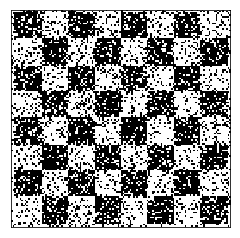
\includegraphics[width = 3.5cm]{images/chessSNP.png}} }
    \qquad
    \subfloat{{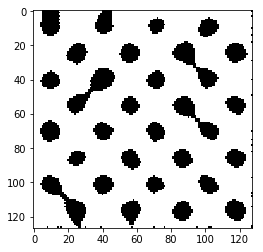
\includegraphics[width = 3.5cm]{images/chessboardfinal.png}} }
    \caption{}
    \label{fig:chessboard}%
\end{figure}

\begin{figure}
    \centering
    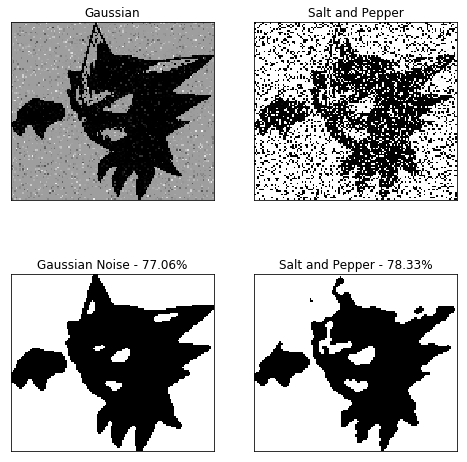
\includegraphics[width = 80mm]{images/ICMFinal.png}
    \caption{Caption}
    \label{fig:ICMfinal}
\end{figure}

Looking at figure \ref{fig:ICMgraph}, it is clear that ICM makes the vast majority of its changes in the first iteration and then quickly reaches a local maximum. In terms of accuracy, ICM fails to maintain the finer details of the image but preserves the general structure rather well while eliminating the salt and pepper noise. 

"To be clear, Iterated Conditional Modes is a coordinate ascent algorithm, and as such, it can only locally optimise the posterior — there is no guarantee of finding a global maximum. Thus if the posterior manifold contains many local maxima, then ICM will be sensitive to initialisation and may perform poorly. Random restarts may mitigate the problem."

\textbf{Question 2}\\
In an attempt to obtain better results, we implemented the Gibbs Sampling Ising Model. This is an example of a Markov Chain Monte Carlo method, meaning THINGSS. After implementing the algorithm, one must decide how to implement the prior and likelihood term from the equation. The prior belief is simply that the value of a pixel is similar to its neighbours, and the likelihood gives that $\textbf{y}_i$ and $\textbf{x}_i$ should be similar. 


For the likelihood function, we used Equation \ref{eq:GibbLikelihood}.
\begin{equation}
    p(\textbf{y}_i |\ \textbf{x}_i) = \exp(\eta \mathcal{L}_i (\textbf{x}_i, \textbf{y}_i))
    \label{eq:GibbLikelihood}
\end{equation}
Intuitively,  $\mathcal{L}_i$ should be defined so that the function would give a larger value for more similar $\textbf{x}_i$ and $\textbf{y}_i$. One such function that satisfies this requirement is 

\begin{equation}
    \mathcal{L}_i = \frac{1}{|\textbf{x}_i - \textbf{y}_i|}
\end{equation}

As we cannot divide by zero, $\textbf{x}_i$ and $\textbf{y}_i$ should never be equal. To avoid this, we use values of 1.1. and -0.1 for $\textbf{x}_i$ in place of 1 and 0.

For the prior, we use something of them form of Equation \ref{eq:GibbPrior}.
\begin{equation}
    \label{eq:GibbPrior}
    p(x_i = 1, \textbf{x}_\mathcal{N}_i) = \exp\left({\beta \sum_{j\in\mathcal{N}_i} 1 * \textbf{x}_ j}\right)
\end{equation}

Figure \ref{fig:GibbDifferentLevels} shows the performance on the images with Gaussian and salt and pepper noise, with different noise levels. It performs better with the Gaussian noise much better than with salt and pepper noise.

One noteworthy point is that we use 'percentage match to the clean image' as our measure, in an attempt to evaluate the effectiveness of the denoising. However, this doesn't actually seem like a great metric, as well as being unusable in practice as we clearly would not know the clean image. For example, an all white image would give (in our case) a percentage match of upwards of 50\% - we would much rather be evaluating our results with some kind of measure of 'how much a person thinks it look like the original'. Quantifying this is clearly somewhere between very hard and impossible, so percentage match is what we have gone with. For example, in Figure \ref{fig:GibbDifferentLevels}, the bottom right image is bordering on unrecognisable but only scores 7\% less than the top right, which does look considerably better. 

\begin{figure}
    \centering
    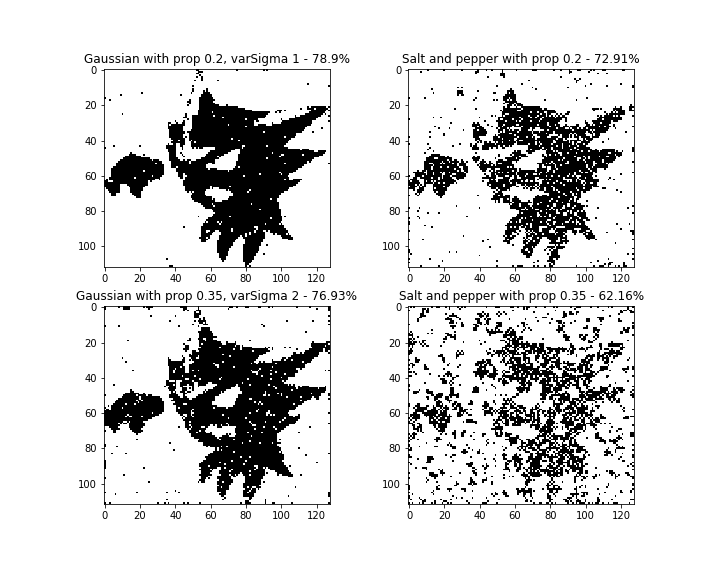
\includegraphics[width=0.48\textwidth]{images/GibbGridDifferentLevels.png}
    \caption{Gibbs results from noise different levels, with percentage match}
    \label{fig:GibbDifferentLevels}
\end{figure}

\textbf{Question 3} \\
We implemented two different methods to change the order in which pixels are visited. The first approach is to shuffle the order in which each pixel is visited for each iteration. With this approach each pixel is still visited once per iteration. This approach has a negligible effect on the performance of the Gibbs sampler, as can be seen in Figure \ref{fig:GibbOrderComp}, but in theory removes any systematic bias that results from visiting pixels in a fixed systematic order each time.

The second approach involves fully randomising which pixels are visited. It is therefore extremely unlikely that each pixel is visited each iteration. This does take longer to converge than our other methods, but ultimately converges to the same result, shown in Figure \ref{fig:GibbOrderComp}.

Figure \ref{fig:GibbOrderHaunter} shows the results of these approaches with their percentage match to the original image. After 50 iterations they give a similar result, and the difference in their matches is effectively negligible and a result of the randomness in the process.
\begin{figure}
    \centering
    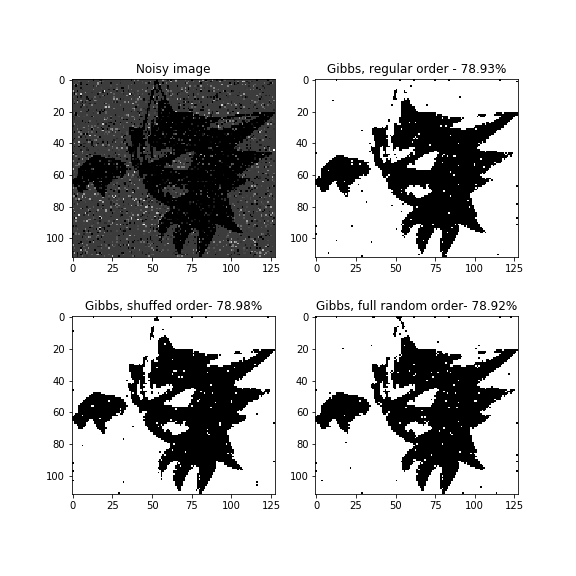
\includegraphics[width=0.48\textwidth]{images/HaunterGibbGridGuassian.png}
    \caption{h a u n t e r}
    \label{fig:GibbOrderHaunter}
\end{figure}
\begin{figure}
    \centering
    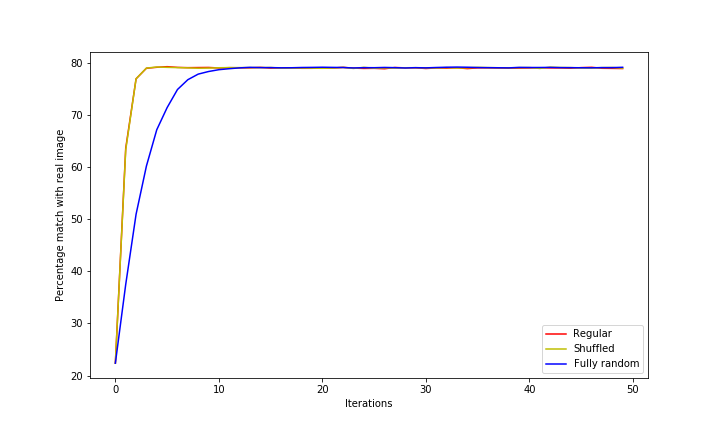
\includegraphics[width=0.48\textwidth]{images/GibbGuassianMatch.png}
    \caption{Graph showing percentage match of different orders for Gibbs applied to our image with Guassian noise, against iterations}
    \label{fig:GibbOrderComp}
\end{figure}

\textbf{Question 4}\\
Each approach tends to the same stable point, which in this case, is after approximately 10 iterations. Running past this point yields little or no improvement. The number of iterations to reach this stable point seems to depend on the choice of hyper-parameters - $\eta$ and $\beta$, which also affect the maximum percentage match reached. This problem is then reduced to optimising the hyper-parameters - something that practically is hard, and 'optimised' is dependent upon the bad percentage match metric.

As we have access to the clean image, it is possible to vary the hyper-parameters and see the effect they have on the results, as in Figure \ref{fig:EtaBetaVariation}. The ratio between $\eta$ and $\beta$ - that is, the ratio of the weights assigned to the likelihood and the prior - seems like the more important factor, not their exact values. Figure \ref{fig:EtaBetaVariation} shows how varying these effects Gibbs' accuracy for a set number of iterations and order. However, different images will be 'optimally' denoised by different choices of $\eta$ and $\beta$, thus optimising these parameters with respect to one image is not a good general approach. If this were being implemented in the real world, these hyper-parameters could be learnt from a training set.
\begin{figure}
    \centering
    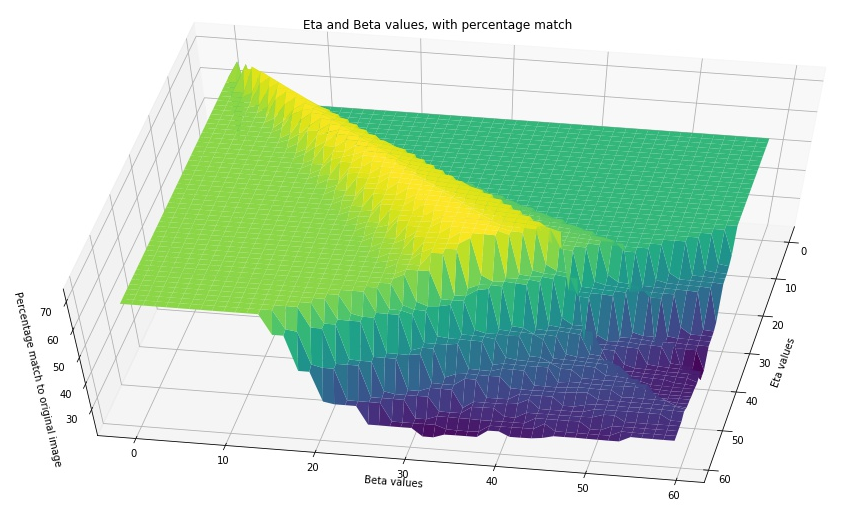
\includegraphics[width=0.48\textwidth]{images/etaBetaResize.png}
    \caption{The effect of varying $\eta$ and $\beta$ on our percentage match}
    \label{fig:EtaBetaVariation}
\end{figure}

\textbf{Question 5}\\
First we consider reverse KL Divergence as this is what is use in the model, defined in Equation \ref{eq:KL_reverse}.
\begin{equation}
     KL(q(\mathbf{x})||p(\mathbf{x})) =  \int q(\mathbf{x}) \log\left(\frac{q(\mathbf{x})}{p(\mathbf{x})}\right)d\textbf{x}
     \label{eq:KL_reverse}
\end{equation}
This shows that the divergence between \qx and \px is weighted by \qx. This gives most divergence at points where we have a probability mass for \qx and small probability mass for \px. Clearly if \q  has no probability mass, then the term is zero, and having \px $=$ \qx also gives zero. Having low \px probability mass gives a small denominator, therefore this combined with some \qx mass contributes to divergence. The resulting KL divergence is therefore a measure of how well \qx fits \px where \qx actually has mass, and does not penalise for sections of \px for which \qx is zero.  

Now consider forward KL divergence - in Equation \ref{eq:KL_forward}.
\begin{equation}
     KL(p(\mathbf{x})||q(\mathbf{x})) = \int p(\mathbf{x})\log\left(\frac{p(\mathbf{x})}{q(\mathbf{x})}\right)d\textbf{x}
     \label{eq:KL_forward}
\end{equation}
Forward KL weights the integral with \px, rather than reverse KL which uses \qx. This means that divergence increases anywhere \px has probability mass, and is increased by low \qx as we are dividing by \qx. This gives large divergence if there are sections of the \px distribution that \qx does not approximate at all, which is - as you'd expect - the opposite of the reverse case. This measure does permit \qx to have extra probability mass far away from \px and this does not count towards divergence, which is the reason this is not useful in our case. (MAYBE USE A GRAPH FOR ILLUSTRATION).

% The difference between these we can also write out, as in Equation \ref{eq:KL_difference}.


% \begin{align}
%     &\int q(\mathbf{x}) \log\left(\frac{q(\mathbf{x})}{p(\mathbf{x})}\right)d\textbf{x} - \int p(\mathbf{x})\log\left(\frac{p(\mathbf{x})}{q(\mathbf{x})}\right)d\textbf{x} \nonumber \\
%     &= \int q(\mathbf{x}) \log q(\mathbf{x})d\textbf{x} + \int p(\mathbf{x}) \log q(\mathbf{x})d\textbf{x} \nonumber \\
%     &\ - \left( \int q(\mathbf{x}) \log p(\mathbf{x})d\textbf{x} + \int p(\mathbf{x}) \log p(\mathbf{x})d\textbf{x} \right) \\
%     &= \int \left( p(\mathbf{x}) + q(\mathbf{x})\right) \log \left( \frac{q(\mathbf{x})}{p(\mathbf{x})}\right)d\textbf{x}
%     \label{eq:KL_difference}
% \end{align}

\textbf{Question 6} By using a mean-field approximation, it is assumed that the approximate distribution over each latent variable is independent. This means that each latent variable is entirely parameterised by an independent parameter $\mu_i$
Hence, the approximate distribution $q(\mathbf{x}$ is entirely parameterised by the parameters $\mu$ for each indiviual latent variable. The parameters $\mu$ parametrise the distribution

Since it is mean-field approximation, each latent variable is 

In the Variational Bayes for Ising Model, the goal is to find the set of parameters $\mu$  each pixel is updated based off two terms.


--------|
|       |
--------| ---------------------------------------|---
|                                                |   |
|                       nice                     |   |
--------|----------------------------------------|---
|       |
--------|

\begin{equation}
    {\mu}_{ij}^{\tau+1} = tanh\left(\sum_{{kl}\epsilon\mathcal{N}(ij)} \omega_{ij}\mu_{kl}^\tau + \frac{1}{2}\left[L_{ij}(1) - L_{ij}(-1)\right] \right)
    \label{eq:variational}
\end{equation}

The first term is the sum of the weighted values of the pixels in the neighbourhood. This term is positively large if the neighbourhood is primarily in agreement with the centre pixel, and negatively large if they are primarily in disagreement. This fits with our intuition, as a positive large value evaluated with $tanh$ will give a value of $1$, similarly $tanh$ will return $-1$ when evaluated with a large negative value. When the pixels in the neighbourhood do not belong primarily to one class, then the summation in equation \ref{eq:variational} is much smaller. As a result the parameter $\mu$, when updated, is affected less by the prior.


The second term in equation 6 is the difference in likelihood of the ij\textsuperscript{th} latent pixel being white or black respectively. This term is large when the observed pixel is black and small when it is white.

In figure \ref{fig:variationalBayes}, it can be seen that the Variational Bayes method performs exceptionally well for Gaussian noise corruption, but less so for "Salt and Pepper" noise. Experimenting with different values of $\eta$ and $\beta$, one could alter how well Variational Bayes performs with the different noises. One configuration of $\eta$ and $\beta$ could perhaps perform well with Gaussian noise but not Salt and Pepper whilst another could do the complete opposite.

\begin{figure}[h]
    \centering
    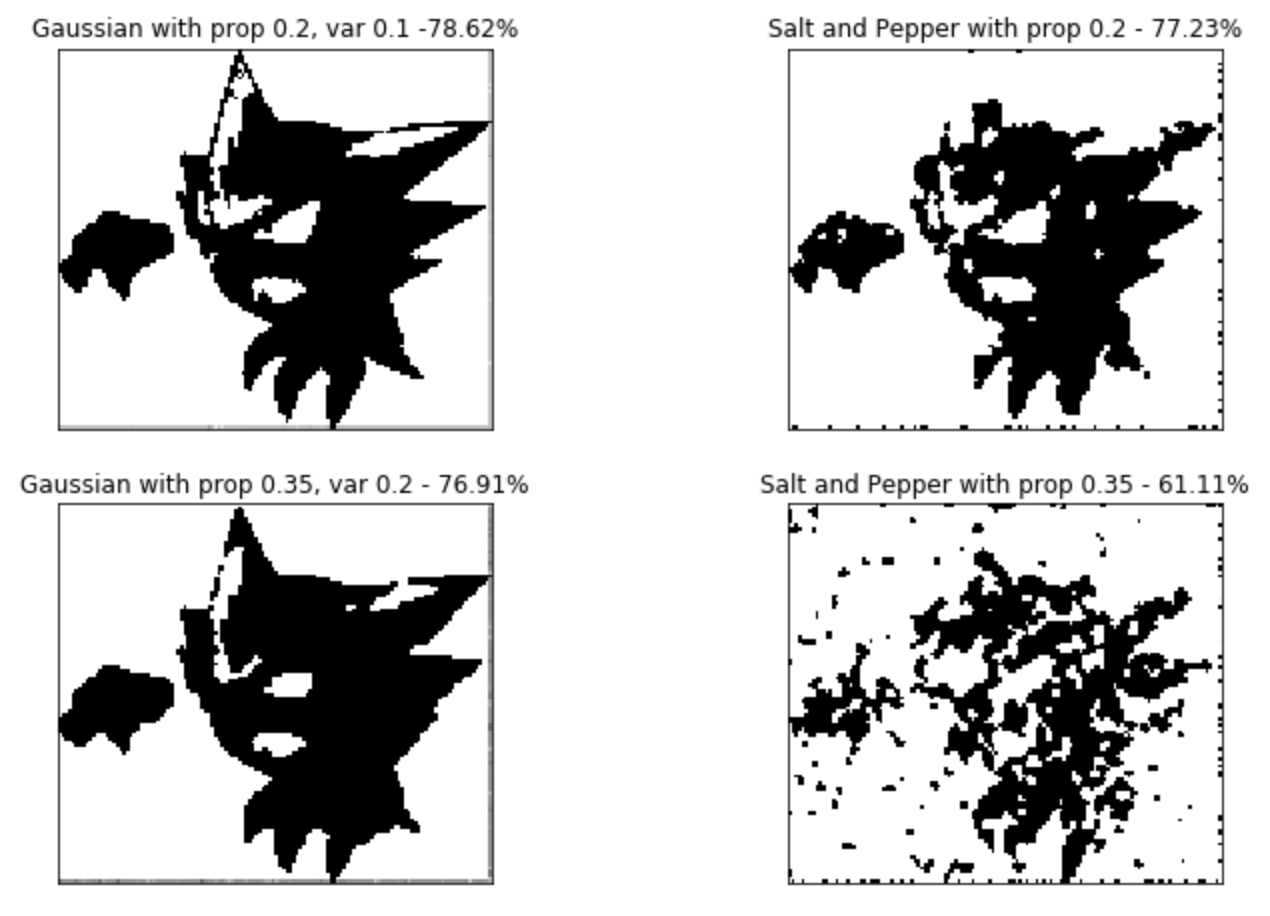
\includegraphics[width=0.48\textwidth]{images/variationalBayes.png}
    \caption{Variational Bayes by Ising Model}
    \label{fig:variationalBayes}
\end{figure}

\textbf{Question 7}
How does the result of the Variational Bayes method compare to the two previous approaches? try to explain the results that you get by relating it to the different methods.\\

Image denoising can be done with a deterministic approach or a stochastic approach. Both variational Bayes and ICM are deterministic, however the former is much more sophisticated in its approach. When comparing the different approaches, it is useful to compare under two categories: time taken to converge, and accuracy. The main takeaway from this


\textbf{Time taken to converge}
Looking at (INSERT FIGURE HERE), it is clear that both ICM and variational Bayes converge faster than Gibbs. 



Iterated Conditional Modes is an example of a coordinate ascent algorithm, which means that it can only optimise the posterior locally and cannot guarantee that a global maximum will be found. The posterior can be viewed as a manifold. If this manifold has many local maxima, then ICM will be sensitive to initialisation and may perform poorly. An intuitive way to think about this problem is to imagine the movement of a ball on a surface with many sinks, and we want the ball to settle in the deepest sinks. Once the ball rolls into one of the sinks (a local minimum) then it cannot leave this local minimum and find the global minimum. The ball will reach different minima dependent on where on the surface it is originally placed. The same problem arises when trying to maximise the posterior in ICM. Random restarts may mitigate the problem and for this reason it may be beneficial to perform ICM by visiting pixels randomly. 

First do a graph of the percentage of original image recovered over time (with the threee methods). We can then use this as a reference for the rest of the question. First compare Variational Bayes to ICM and then compare Variational Bayes to Gibbs. I think the comparison with Gibbs seems important considering he stressed it in the lecture. We should discuss the positives and negatives of both approaches and give situations in which each would be the preferable approach. 

Use a graph to show percentage accuracy, use another graph to show changes per iteration.

\textbf{Question 8}
Implement the image segmentation with one of the inference approaches we have gone through, either the sampling based method or the deterministic approach.\\

%https://github.com/vsmolyakov/experiments_with_python/blob/master/chp02/mean_field_mrf.ipynb








CHECKLIST\\
-------------------\\
Question 1:\\ Put in images and format but otherwise finished
Question 2:\\
Question 3:\\
Question 4:\\
Question 5:\\
Question 6:\\
Question 7:\\
Question 8:\\
Question 9:\\
Question 10:\\
\textbf{Final Thoughts}\\
Final thoughts...\\

LIST OF TODOS\\
-------------------\\
James - fix images for question one, figure out how to calculate the percentage change and graph it. Should be the same as jakes code for the graphing, different for implementing in the ICM function.
//
//
Work together to do question 7. This should probably be the bulkiest part of the report. Go into detail and try to give the intuition behind it as well as the mathematics that are going on under the hood.
//
//
work together to figure out how to do question 8. My guess is that we implement image segmentation with Gibbs or Variational Bayes. ICM would be interesting to try but realistically its so shit i doubt it'd work. If possible try question 8 with both variational Bayes and Gibbs. 
//
//
Have the content and images for questions 1-8 fully finalised before Thursday night. 
//
//
Think about how to structure an abstract and conclusion if we have space (which we might)
%----------------------------------------------------------------------------------------
%	BIBLIOGRAPHY
%----------------------------------------------------------------------------------------

\printbibliography[title={Bibliography}] % Print the bibliography, section title in curly brackets

%----------------------------------------------------------------------------------------

\end{document}
